% vim: set ts=4 sw=4 tw=80 noexpandtab:

\documentclass{42-en}

%******************************************************************************%
%                                                                              %
%                                   Prologue                                   %
%                                                                              %
%******************************************************************************%
\usepackage[
    type={CC},
    modifier={by-nc-sa},
    version={4.0},
]{doclicense}
\usepackage{amsmath} % The amsmath package provides commands to typeset matrices with different delimiters. 
\usepackage{epigraph}
\setlength\epigraphwidth{.95\textwidth}
\usepackage{multirow}
\usepackage{cancel}
%****************************************************************%
%                  Re/definition of commands                     %
%****************************************************************%

\newcommand{\ailogo}[1]{\def \@ailogo {#1}}\ailogo{assets/42ai_logo.pdf}

%%  Redefine \maketitle
\makeatletter
\def \maketitle {
  \begin{titlepage}
    \begin{center}
	%\begin{figure}[t]
	  %\includegraphics[height=8cm]{\@ailogo}
	  
\includegraphics[height=8cm]{assets/42ai_logo.pdf}
	%\end{figure}
      \vskip 5em
      {\huge \@title}
      \vskip 2em
      {\LARGE \@subtitle}
      \vskip 4em
    \end{center}
    %\begin{center}
	  %\@author
    %\end{center}
	%\vskip 5em
  \vfill
  \begin{center}
    \emph{\summarytitle : \@summary}
  \end{center}
  \vspace{2cm}
  %\vskip 5em
  %\doclicenseThis
  \end{titlepage}
}
\makeatother

\makeatletter
\def \makeheaderfilesforbidden
{
  \noindent
  \begin{tabularx}{\textwidth}{|X X  X X|}
    \hline
  \multicolumn{1}{|>{\raggedright}m{1cm}|}
  {\vskip 2mm 
\includegraphics[height=1cm]{assets/42ai_logo.pdf}} &
  \multicolumn{2}{>{\centering}m{12cm}}{\small Exercise : \@exnumber } &
  \multicolumn{1}{ >{\raggedleft}p{1.5cm}|}
%%              {\scriptsize points : \@exscore} \\ \hline
              {} \\ \hline

  \multicolumn{4}{|>{\centering}m{15cm}|}
              {\small \@extitle} \\ \hline

  \multicolumn{4}{|>{\raggedright}m{15cm}|}
              {\small Turn-in directory : \ttfamily
                $ex\@exnumber/$ }
              \\ \hline
  \multicolumn{4}{|>{\raggedright}m{15cm}|}
              {\small Files to turn in : \ttfamily \@exfiles }
              \\ \hline

  \multicolumn{4}{|>{\raggedright}m{15cm}|}
              {\small Forbidden functions : \ttfamily \@exforbidden }
              \\ \hline

%%  \multicolumn{4}{|>{\raggedright}m{15cm}|}
%%              {\small Remarks : \ttfamily \@exnotes }
%%              \\ \hline
\end{tabularx}
%% \exnotes
\exrules
\exmake
\exauthorize{None}
\exforbidden{None}
\extitle{}
\exnumber{}
}
\makeatother

%%  Syntactic highlights
\makeatletter
\newenvironment{pythoncode}{%
  \VerbatimEnvironment
  \usemintedstyle{emacs}
  \minted@resetoptions
  \setkeys{minted@opt}{bgcolor=black,formatcom=\color{lightgrey},fontsize=\scriptsize}
  \begin{figure}[ht!]
    \centering
    \begin{minipage}{16cm}
      \begin{VerbatimOut}{\jobname.pyg}}
{%[
      \end{VerbatimOut}
      \minted@pygmentize{c}
      \DeleteFile{\jobname.pyg}
    \end{minipage}
\end{figure}}
\makeatother

\usemintedstyle{native}

\begin{document}

% =============================================================================%
%                     =====================================                    %

\title{Machine Learning Bootcamp - Module 03}
\subtitle{Logistic Regression}
\author{
  Maxime Choulika (cmaxime), Pierre Peigné (ppeigne), Matthieu David (mdavid), Amir Mahla (amahla), Mathieu Perez (maperez)
}

\summary
{
  Discover your first classification algorithm: logistic regression.
  You will learn about its loss function, gradient descent and some metrics to evaluate its performance.
}

\maketitle
%******************************************************************************%
%                                                                              %
%                        Section usefull ressources                            %
%                          for ML Modules                                      %
%                                                                              %
%******************************************************************************%


\chapter*{Notions and ressources}

\section*{Notions of the module}
Sum, mean, variance, standard deviation, vectors and matrices operations.  
Hypothesis, model, regression, loss function. 

\section*{Useful Ressources}

You are strongly advise to use the following resource:
\href{https://www.coursera.org/learn/machine-learning}{Machine Learning MOOC - Stanford}
These videos are available at no cost; simply log in, select "Enroll for Free", then click "Audit" at the bottom of the pop-up window.
The following sections of the course are pertinent to today's exercises: 

\newpage

\subsection*{Week 1: Introduction to Machine Learning}

\subsubsection*{Supervised vs. Unsupervised Machine Learning}
\begin{itemize}
  \item What is Machine Learning?
  \item Supervised Learning Part 1
  \item Supervised Learning Part 2
  \item Unsupervised Learning Part 1
  \item Unsupervised Learning Part 2
\end{itemize}
    
\subsubsection*{Regression Model}  
\begin{itemize}
  \item Regression Model Part 1
  \item Regression Model Part 2
  \item Cost Function Formula
  \item Cost Function Intuition
  \item Visualizing the cost function
  \item Visualizing Example
  \item \textit{Keep what remains for tomorow ;)}
\end{itemize}

\emph{All videos above are available also on this \href{https://youtube.com/playlist?list=PLkDaE6sCZn6FNC6YRfRQc_FbeQrF8BwGI&feature=shared}{Andrew Ng's YouTube playlist} from 3 to 14 includes}

\subsubsection*{Linear Algebra Review}
\begin{itemize}
  \item \href{https://www.youtube.com/watch?v=XMB__E658fQ}{Matrices and Vectors}
  \item \href{https://www.youtube.com/watch?v=k1JGJhUGmBE}{Addition and Scalar Multiplication}
  \item \href{https://www.youtube.com/watch?v=VIfykceJoZI}{Matrix Vector Multiplication}
  \item \href{https://www.youtube.com/watch?v=JHZKyt0m1kc}{Matrix Matrix Multiplication}
  \item \href{https://www.youtube.com/watch?v=wqM7O_ZUtCc}{Matrix Multiplication Properties}
  \item \href{https://www.youtube.com/watch?v=IUf8HDyUeY0}{Inverse and Transpose}
\end{itemize}

%******************************************************************************%
%                                                                              %
%                        Common Instructions                                   %
%                          for Python Projects                                 %
%                                                                              %
%******************************************************************************%

\chapter{Common Instructions}
\begin{itemize}
  \item The version of Python recommended to use is 3.7, you can
  check the version of Python with the following command: \texttt{python -V}
  
  \item The norm: during this bootcamp, it is recommended to follow the
  \href{https://www.python.org/dev/peps/pep-0008/}{PEP 8 standards}, though it is not mandatory.
  You can install \href{https://pypi.org/project/pycodestyle}{pycodestyle} which
  is a tool to check your Python code.
  \item The function \texttt{eval} is never allowed.
  \item The exercises are ordered from the easiest to the hardest.
  \item Your exercises are going to be evaluated by someone else,
  so make sure that your variable names and function names are appropriate and civil.
  \item Your manual is the internet.
  
  \item If you are a student from 42, you can access our Discord server 
  on \href{https://discord.com/channels/887850395697807362/887850396314398720}{42 student's associations portal} and ask your
  questions to your peers in the dedicated Bootcamp channel. 

  \item You can learn more about 42 Artificial Intelligence by visiting \href{https://42-ai.github.io}{our website}.

  \item If you find any issue or mistake in the subject please create an issue on \href{https://github.com/42-AI/bootcamp_machine-learning/issues}{42AI repository on Github}.
  
  \item We encourage you to create test programs for your
  project even though this work \textbf{won't have to be
  submitted and won't be graded}. It will give you a chance
  to easily test your work and your peers’ work. You will find
  those tests especially useful during your defence. Indeed,
  during defence, you are free to use your tests and/or the
  tests of the peer you are evaluating.

  \item We are constantly looking to improve these bootcamps, and your feedbacks are essential for us to do so !\\
  You can tell us more about your experience with this module by filling \href{https://forms.gle/ruP9wv1RfwbneKJE8}{this form}.\\
  Thank you in advance and good luck for this bootcamp !

\end{itemize}
\newpage
\tableofcontents
\startexercices

%                     =====================================                    %
% =============================================================================%


%******************************************************************************%
%                                                                              %
%                                   Exercises                                  %
%                                                                              %
%******************************************************************************%

% ============================================== %
% ===========================(start ex 00)       %
\chapter{Exercise 00}
%******************************************************************************%
%                                                                              %
%                                 Interlude                                    %
%                         for Machine Learning module                          %
%                                                                              %
%******************************************************************************%

% =============================== %
\section*{Interlude}
% =============================== %
\subsection*{Classification: The Art of Labelling Things}
% ******************************* %
Over the last three modules you have implemented your first machine learning algorithm.\\
\\
You are now familiar the three-steps cycle we follow when we build \textbf{learning algorithms}:
\\
\begin{figure}[!h]
    \centering
    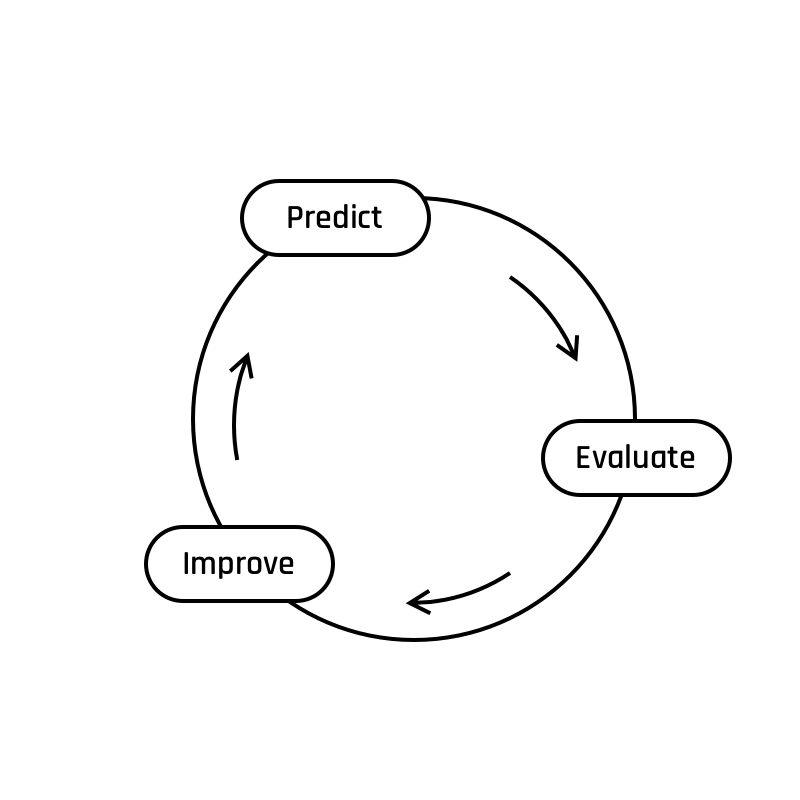
\includegraphics[scale=0.25]{assets/Default.png}
    %\caption{The Learning Cycle}
\end{figure}
\\
The first algorithm you discovered, \textbf{Multivariate Linear Regression}, can now be used to predict a numerical value, based on several features.
This algorithm uses gradient descent to optimize its loss function.\\
\\
Now let's introduce your first \textbf{classification algorithm}: the notorious \textbf{Logistic Regression.}
\hint{regression vs classification; discrete vs continuous values}
\newpage
\noindent{\textbf{Logistic regression} performs a \textit{classification task}, which means that you are not predicting a numerical value (like price, age, grades...) 
but \textbf{categories}, or \textbf{labels} (like dog, cat, sick/healty...)}.
\\
\warn{
    Don't be confused by the word \textit{'regression'} in \textbf{Logistic Regression}.
    It really is a \textit{classification task}! The name is a bit tricky but you will quickly get used to it.
    Once again: \textbf{Logistic Regression is a classification algorithm} which assigns a label/category/class to a given example.
}
\info{
    In this module we will use the following terms interchangeably: \textbf{class}, \textbf{category}, and \textbf{label}.
    They all refer to the \textit{groups} to which each training example can be assigned to, in a classification task.
}

% =============================== %
\subsection*{Predict I: Introducing the Sigmoid Function}
% ******************************* %

\begin{figure}[!h]
    \centering
    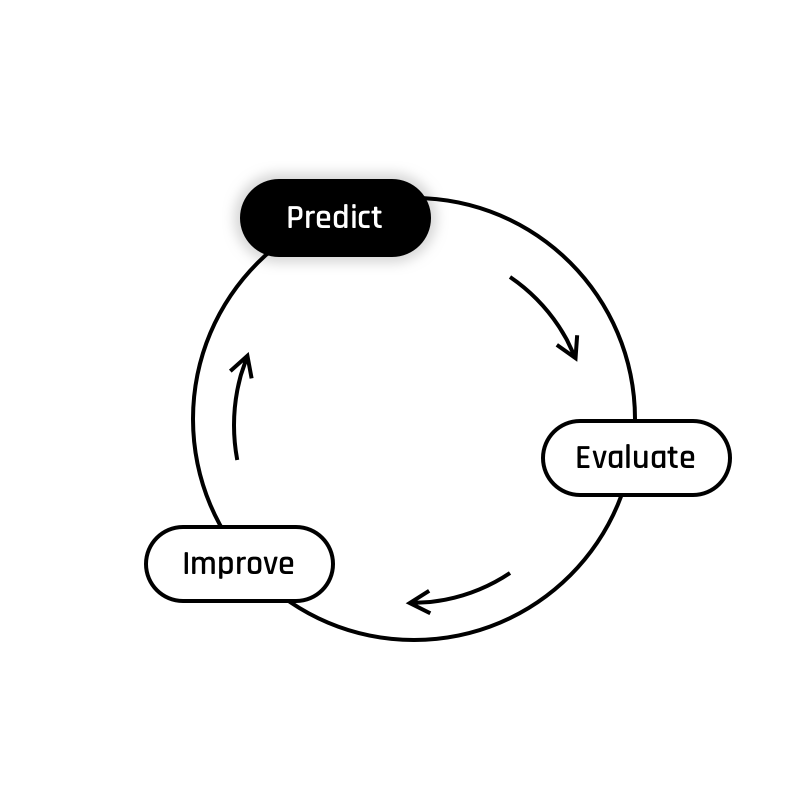
\includegraphics[scale=0.25]{assets/Predict.png}
    %\caption{The Learning Cycle - Predict}
\end{figure}

% =============================== %
\subsubsection*{Formulating a Hypothesis}
% ******************************* %
Remember that a hypothesis, denoted $h(\theta)$, is an equation that combines a set of \textbf{features} (that characterizes an example) with \textbf{parameters} in order to output a \textbf{prediction}.\\
\\
Remember the hypothesis we used in linear regression?\\
$$
h(\theta) = \theta_0 + \theta_{1} x_{1}^{(i)} + \dots + \theta_{n} x_{n}^{(i)} = \theta \cdot x'^{(i)}
$$
\newline
It worked fine to predict continuous values, but could we also use it to tell, for example, 
if a patient is sick or not?
That's a yes-or-no question, so the output from the hypothesis function should reflect that.\\
\\
To get started, we will assign each class a numerical value: sick patients will be 
assigned a value of 1, and healthy patients will be assigned a value of 0.\\
The goal will be to build a hypothesis that outputs a probability that a patient is sick as a float number in the range of [0, 1].\\
\\
The good news is that we can keep the linear equation we already worked with!\\
\\
All we need to do is squash its output through another function that is bounded between 0 and 1.\\
\\
That's the purpose of the \textbf{Sigmoid function} and your next assignment is to implement it!

\newpage
\extitle{Sigmoid}
\turnindir{ex00}
\exnumber{00}
\exfiles{sigmoid.py}
\exforbidden{None}
\makeheaderfilesforbidden

% ================================== %
\section*{Objective}
% ---------------------------------- %
Introduction to the hypothesis in the case of logistic regression.
You must implement the sigmoid function, given by the following formula:  

$$
\text{sigmoid}(x) = \cfrac{1} {1 + e^{-x}}
$$

Where:
\begin{itemize}
  \item $x$ is a scalar or a vector,
  \item $e$ is the contracted form for exponential function. It is also a mathematical constant, named Euler's number.
\end{itemize}

This function is also known as \textbf{Standard logistic sigmoid function}.
This explains the name \textit{logistic regression}.

The sigmoid function transforms an input into a probability value, i.e. a value between 0 and 1.  
This probability value will then be used to classify the inputs.

% ================================== %
\section*{Instructions}
% ---------------------------------- %
In the \texttt{sigmoid.py} file, write the following function as per the instructions below:

\par

\begin{minted}[bgcolor=darcula-back,formatcom=\color{lightgrey},fontsize=\scriptsize]{python}
def sigmoid_(x):
    """
    Compute the sigmoid of a vector.
    Args:
        x: has to be a numpy.ndarray of shape (m, 1).
    Returns: 
        The sigmoid value as a numpy.ndarray of shape (m, 1).
        None if x is an empty numpy.ndarray.
    Raises:
        This function should not raise any Exception.
    """
    ... Your code ...
\end{minted}

% ================================== %
\section*{Examples}
% ---------------------------------- %

\begin{minted}[bgcolor=darcula-back,formatcom=\color{lightgrey},fontsize=\scriptsize]{python}
# Example 1:
x = np.array([[-4]])
sigmoid_(x)
# Output:
array([[0.01798620996209156]])

# Example 2:
x = np.array([[2]])
sigmoid_(x)
# Output:
array([[0.8807970779778823]])

# Example 3:
x = np.array([[-4], [2], [0]])
sigmoid_(x)
# Output:
array([[0.01798620996209156], [0.8807970779778823], [0.5]])
\end{minted}


\info{
  Our sigmoid formula is a special case of the logistic function below, with $L = 1$, $k = 1$ and $x_0 = 0$:
  $$
  f(x) = \cfrac{L}{1 + e^{-k(x-x_0)}}
  $$
}
% ===========================(fin ex 00)         %
% ============================================== %
\newpage
% ===========================(start ex 01)       %
\chapter{Exercise 01}
%******************************************************************************%
%                                                                              %
%                                 Interlude                                    %
%                         for Machine Learning module                          %
%                                                                              %
%******************************************************************************%

% =============================== %
\section*{Linear Algebra Tricks part II}
% ******************************* %

If you tried to run your code on a very large dataset, you would find that it sometimes takes a (very) long time to execute!
That's because it doesn't use the power of Python libraries that are optimized for matrix operations.\\
\newline
Remember the linear algebra trick from the previous module? Let's use it again!  
If you concatenate a column of $1$'s to the left of the $x$ vector, you get what we called matrix $X'$.   
$$
X' = \begin{bmatrix} 1 & x^{(1)} \\ \vdots & \vdots \\ 1 & x^{(m)}\end{bmatrix}
$$
This transformation is very convenient because we can rewrite each $1$ as $x_0^{(i)}$, and each $x^{(i)}$ as $x_1^{(i)}$.
So now the $X'$ matrix looks like this:
$$
X' = \begin{bmatrix} x_0^{(1)} & x_1^{(1)} \\ \vdots & \vdots \\ x_0^{(m)} & x_1^{(m)}\end{bmatrix}
$$
Notice that each $x^{(i)}$ example becomes a vector made of $(x^{(i)}_0, x^{(i)}_1)$.  
The $0$ and $1$ indices on the $x$ features correspond to the indices of the $\theta$ parameters with which they will be multiplied.\\
\newline
Why does this matter?
Well, if we take the equation from the previous exercise:

$$
\nabla(J)_0 = \frac{1}{m}\sum_{i=1}^{m}(h_{\theta}(x^{(i)}) - y^{(i)})
$$
We can multiply it by $1$ without changing its value:
$$
\nabla(J)_0 = \frac{1}{m}\sum_{i=1}^{m}(h_{\theta}(x^{(i)}) - y^{(i)}) \cdot 1
$$
And rewrite $1$ as $x_0^{(i)}$:
$$
\nabla(J)_0 = \frac{1}{m}\sum_{i=1}^{m}(h_{\theta}(x^{(i)}) - y^{(i)})x_{0}^{(i)}
$$
This means that the equation for $\nabla(J)_0$ is now similar to the equation we had for $\nabla(J)_1$, so they can both be captured by ONE \textbf{generic equation}:
$$
\begin{matrix}
\nabla(J)_j = \frac{1}{m}\sum_{i=1}^{m}(h_{\theta}(x^{(i)}) - y^{(i)})x_{j}^{(i)} & & \text{ for j = 0, 1}    
\end{matrix}
$$
And as you probably suspected, a generic equation opens the door to vectorization...

% =============================== %
\subsection*{Vectorizing the Gradient Calculation}
% ******************************* %
Now it's time to learn how to calculate the entire gradient in one short, pretty, linear algebra equation!  
\begin{itemize}
    \item First, we'll use the $X'$ matrix and our vectorized hypothesis equation $h_{\theta}(x)=X'\theta$
    $$
    \begin{matrix}
    \nabla(J)_j = \frac{1}{m} (X'\theta - y)X'_{j} & & \text{ for j = 0, 1}
    \end{matrix}
    $$
    
    \item Second, we need to tweak the equation a bit so that it directly returns a $\nabla(J)$ vector containing both $\nabla(J)_0$ and $\nabla(J)_1$.
    
    $$
    \nabla(J) = \frac{1}{m} {X'}^T(X'\theta - y)    
    $$
\end{itemize}
If the equation does not seems obvious, play a bit with your vectors, on paper and in your code, until you get it.\\

% =============================== %
\subsubsection*{Notation Remark}
% ******************************* %
${X'}^T$: You might wonder what the $^T$ is for.
It means the $X'$ matrix must be \textbf{transposed}.\\
\newline
Transposing a matrix flips it on its diagonal so that its rows become its columns and \textit{vice-versa}.
Here we need to make sure that matrix dimensions are appropriate and allow for multiplication, and to multiply the right items together.
\newpage
\extitle{Logistic Hypothesis}
\turnindir{ex01}
\exnumber{01}
\exfiles{log\_pred.py}
\exforbidden{None}
\makeheaderfilesforbidden

% ================================= %
\section*{Objective}
% --------------------------------- %
Introduction to the hypothesis notion in the context of logistic regression.\\
\\
You must implement the following formula as a function:\\

$$
\begin{matrix}
\hat{y} & = & \text{sigmoid}(X' \cdot \theta) & = & \cfrac{1} {1 + e^{-X' \cdot \theta}}    
\end{matrix}
$$
Where:
\begin{itemize}
  \item $X$ is a matrix of dimensions $(m \times n)$, the design matrix
  \item $X'$ is a matrix of dimensions $(m \times (n + 1))$, 
  the design matrix onto which a column of $1$'s is added as a first column
  \item $\hat{y}$ is a vector of dimension $m$, the vector of predicted values
  \item $\theta$ is a vector of dimension $(n + 1)$, the vector of parameters
\end{itemize}
Be careful: 
\begin{itemize}
  \item the $x$ your function will get as an input corresponds to $X$, the $(m \times n)$ matrix.
        Not $X'$.
  \item $\theta$ is a vector of length $(n + 1)$
\end{itemize}
\newpage
% ================================= %
\section*{Instructions}
% --------------------------------- %
In the \texttt{log\_pred.py} file, write the following function as per the instructions below:\\
\par
\begin{minted}[bgcolor=darcula-back,formatcom=\color{lightgrey},fontsize=\scriptsize]{python}
def logistic_predict_(x, theta):
    """Computes the vector of prediction y_hat from two non-empty numpy.ndarray.
    Args:
      x: has to be an numpy.ndarray, a vector of dimension m * n.
      theta: has to be an numpy.ndarray, a vector of dimension (n + 1) * 1.
    Returns:
      y_hat as a numpy.ndarray, a vector of dimension m * 1.
      None if x or theta are empty numpy.ndarray.
      None if x or theta dimensions are not appropriate.
    Raises:
      This function should not raise any Exception.
    """
    ... Your code ...
\end{minted}

% ================================= %
\section*{Examples}
% --------------------------------- %

\begin{minted}[bgcolor=darcula-back,formatcom=\color{lightgrey},fontsize=\scriptsize]{python}
# Example 1
x = np.array([4]).reshape((-1, 1))
theta = np.array([[2], [0.5]])
logistic_predict_(x, theta)
# Output: 
array([[0.98201379]])

# Example 1
x2 = np.array([[4], [7.16], [3.2], [9.37], [0.56]])
theta2 = np.array([[2], [0.5]]) 
logistic_predict_(x2, theta2)
# Output: 
array([[0.98201379],
       [0.99624161],
       [0.97340301],
       [0.99875204],
       [0.90720705]])

# Example 3
x3 = np.array([[0, 2, 3, 4], [2, 4, 5, 5], [1, 3, 2, 7]])
theta3 = np.array([[-2.4], [-1.5], [0.3], [-1.4], [0.7]])
logistic_predict_(x3, theta3)
# Output: 
array([[0.03916572],
       [0.00045262],
       [0.2890505 ]])
\end{minted}
% ===========================(fin ex 01)         %
% ============================================== %
\newpage
% ============================================== %
% ===========================(start ex 02)       %
\chapter{Exercise 02}
%******************************************************************************%
%                                                                              %
%                                 Interlude                                    %
%                         for Machine Learning module                          %
%                                                                              %
%******************************************************************************%

\section*{Interlude - Predict, Evaluate, Improve}

\epigraph
{A computer program is said to learn from experience E, with respect to some
class of tasks T, and performance measure P, if its performance at tasks in T,
as measured by P, improves with experience E.}{\textit{Tom Mitchell,\\Machine Learning, 1997}}

\begin{quote}{}

\end{quote}

In other words to learn you have to improve.\\
To improve you have to evaluate your performance.\\
To evaluate your performance you need to start performing on the task you want to be good at.


One of the most common tasks in Machine Learning is \textbf{prediction}.\\  
This will be your algorithm's task.\\
This will be your task.  

\begin{figure}[h!]
  \centering
  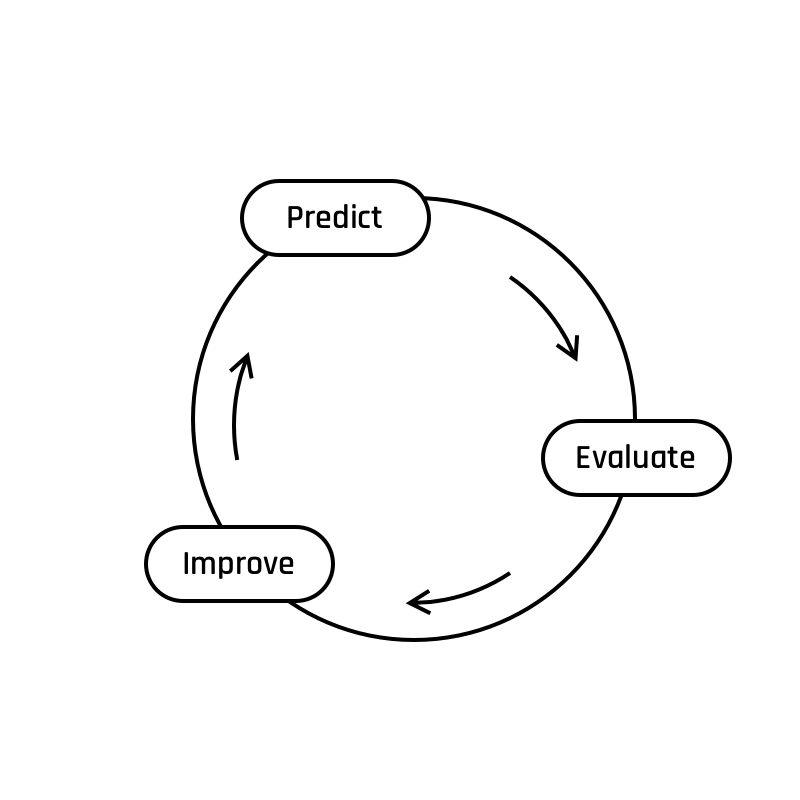
\includegraphics[scale=0.25]{assets/Default.png}
  \caption{cycle neutral}
\end{figure}

\section*{Predict}

\begin{figure}[h!]
  \centering
  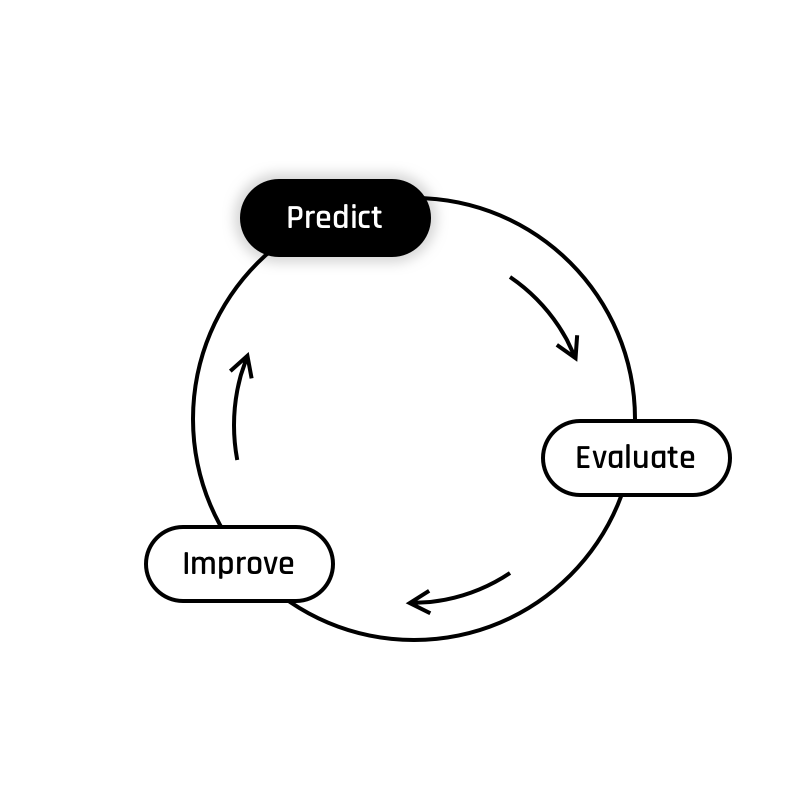
\includegraphics[scale=0.25]{assets/Predict.png}
  \caption{cycle predict}
\end{figure}

\subsection*{A very simple model}

We have some data. We want to model it.  
\begin{itemize}
    \item First we need to \textit{make an assumption}, or hypothesis, \textit{about the structure of the data and the relationship between the variables}.  
    \item Then we can \textit{apply that hypothesis to our data to make predictions}.
\end{itemize}

$$
hypothesis(data) = predictions
$$

\subsubsection*{Hypothesis}
Let's start with a very simple and intuitive \textbf{hypothesis} on how the price of a spaceship can be predicted based on the power of its engines.\\
We will consider that \textit{the more powerful the engines are, the more expensive the spaceship is}.\\
Furthermore, we will assume that the price increase is \textbf{proportional} to the power increase. In other words, we will look for a \textbf{linear relationship} between the two variables.

This means that we will formulate the price prediction with a \textbf{linear equation}, that you might be already familiar with:

$$
\hat{y} = ax + b
$$

We add the \texttt{\^} symbol over the $y$ to specify that $\hat{y}$ \textit{(pronounced y-hat)} is a \textbf{prediction} (or estimation) of the real value of $y$. The prediction is calculated with the \textbf{parameters} $a$ and $b$ and the input value $x$.

For example, if $a = 5$ and $b = 33$, then $\hat{y} = 5x + 33$.

But in Machine Learning, we don't like using the letters $a$ and $b$. Instead we will use the following notation:

$$
\hat{y} = \theta_0 + \theta_1 x
$$

So if $\theta_0 = 33$ and $\theta_1 = 5$, then $\hat{y} = 33+ 5x$.

To recap, this linear equation is our \textbf{hypothesis}. Then, all we will need to do is find the right values for our parameters $\theta_0$ and $\theta_1$ and we will get a fully-functional prediction \textbf{model}.


\subsubsection*{Predictions}
Now, how can we generate a set of predictions on an entire dataset? Let's consider a dataset containing $m$ data points (or space ships), called \textbf{examples}.

What we do is stack the $x$ and $\hat{y}$ values of all examples in vectors of length $m$. The relation between the elements in our vectors can then be represented with the following formula:

$$
\begin{matrix}
\hat{y}^{(i)} = \theta_0 + \theta_1 x^{(i)} & & \text{ for i = 1, ..., m}
\end{matrix}
$$  

Where:
\begin{itemize}
    \item $\hat{y}^{(i)}$ is the $i^{th}$ component of vector $y$
    \item $x^{(i)}$ is the $i^{th}$ component of vector $x$   
\end{itemize}

Which can be experessed as:

$$
\hat{y} = \begin{bmatrix}\theta_0 + \theta_1 \times x^{(1)} \\ \vdots \\  \theta_0 + \theta_1 \times x^{(m)}\ \end{bmatrix}
$$  

For example,

$$
\text{given } \theta = \begin{bmatrix}33 \\ 5 \end{bmatrix} \text{ and } x = \begin{bmatrix}1 \\ 3 \end{bmatrix} \text{: }
$$

$$
\hat{y} = h_{\theta}(x) = \begin{bmatrix} 33 +  5 \times 1 \\ 33 + 5 \times 3\end{bmatrix}  = \begin{bmatrix} 38 \\ 48 \end{bmatrix} 
$$

\newpage

\subsection*{More information}

\subsubsection*{Why the $\theta$ notation?}

You might have two questions at the moment:
\begin{itemize}
    \item \textbf{WTF is that weird  symbol?}
    This strange symbol, $\theta$, is called "theta".
    
    \item \textbf{Why use this notation instead of $a$ and $b$, like we're used to?}
    Despite its seeming more complicated at first, the theta notation is actually meant to simplify your equations later on. Why?
    $a$ and $b$ are good for a model with two parameters, but you will soon need to build more complex models that take into account more variables than just $x$.
    You could add more letters like this:  $\hat{y} = ax_1 + bx_2 + cx_3 + ... + yx_{25} + z$  
    But how do you go beyond 26 parameters? And how easily can you tell what parameter is associated with, let's say, $x_{19}$? That's why it becomes more handy to describe all your parameters using the theta notation and indices.
    With $\theta$, you just have to increment the number to name the parameter:
    $\hat{y} = \theta_0 + \theta_1 x_1 + \theta_2 x_2 + ... + \theta_{2468} x_{2468}$ ... Easy right?
\end{itemize}


\subsubsection*{Another common notation}

$$
\begin{matrix} & & \hat{y} & = & h_{\theta}(x)\end{matrix}
$$

Because $\hat{y}$ is calculated with our linear hypothesis using $\theta$ and $x$, it is sometimes written as $h_{\theta}(x)$.
The $h$ stands for \textit{hypothesis}, and can be read as \textit{"the result of our hypothesis h given x and theta"}.

Then if $x = 7$, we can calculate:
$\hat{y} = h_{\theta}(x) = 33 + 5 \times 7 = 68$
We can now say that according to our linear model, the \textbf{predicted value} of $y$ given ($x = 7$) is 68.

\newpage
\extitle{Logistic Loss Function}
\turnindir{ex02}
\exnumber{02}
\exfiles{log\_loss.py}
\exforbidden{None}
\makeheaderfilesforbidden

% ================================= %
\section*{Objective}
% --------------------------------- %
Understanding and manipulation of the loss function concept in the case of logistic regression.
You must implement the following formula as a function:  

$$
J( \theta) = -\cfrac{1} {m} \lbrack \sum_{i = 1}^{m} y^{(i)}\log(\hat{y}^{(i)})) + (1 - y^{(i)})\log(1 - \hat{y}^{(i)})\rbrack
$$

Where:
\begin{itemize}
  \item $\hat{y}$ is a vector of dimension $m$, the vector of predicted values,
  \item $\hat{y}^{(i)}$ is the $i^{th}$ component of the $\hat{y}$ vector,
  \item $y$ is a vector of dimension $m$, the vector of expected values,
  \item $y^{(i)}$ is the $i^{th}$ component of the $y$ vector.
\end{itemize}


% ================================= %
\section*{Instructions}
% --------------------------------- %
In the \texttt{log\_loss.py} file, write the following function as per the instructions below:
\par
\begin{minted}[bgcolor=darcula-back,formatcom=\color{lightgrey},fontsize=\scriptsize]{python}
def log_loss_(y, y_hat, eps=1e-15):
    """
    Computes the logistic loss value.
    Args:
        y: has to be an numpy.ndarray, a vector of shape m * 1.
        y_hat: has to be an numpy.ndarray, a vector of shape m * 1.
        eps: has to be a float, epsilon (default=1e-15)
    Returns:
        The logistic loss value as a float.
        None on any error.
    Raises:
        This function should not raise any Exception.
    """
    ... Your code ...
\end{minted}

\hint{
  The logarithmic function isn't defined in $0$.  
  This means that if $y^{(i)} = 0$ you will get an error when you try to compute $log(y^{(i)})$.
  The purpose of the \texttt{eps} argument is to avoid $log(0)$ errors.
  It is a very small residual value we add to \texttt{y}.
}

% ================================= %
\section*{Examples}
% --------------------------------- %
\begin{minted}[bgcolor=darcula-back,formatcom=\color{lightgrey},fontsize=\scriptsize]{python}
# Example 1:
y1 = np.array([1]).reshape((-1, 1))
x1 = np.array([4]).reshape((-1, 1))
theta1 = np.array([[2], [0.5]])
y_hat1 = logistic_predict_(x1, theta1)
log_loss_(y1, y_hat1)
# Output:
0.01814992791780973

# Example 2:
y2 = np.array([[1], [0], [1], [0], [1]])
x2 = np.array([[4], [7.16], [3.2], [9.37], [0.56]])
theta2 = np.array([[2], [0.5]])
y_hat2 = logistic_predict_(x2, theta2)
log_loss_(y2, y_hat2)
# Output:
2.4825011602474483

# Example 3:
y3 = np.array([[0], [1], [1]])
x3 = np.array([[0, 2, 3, 4], [2, 4, 5, 5], [1, 3, 2, 7]])
theta3 = np.array([[-2.4], [-1.5], [0.3], [-1.4], [0.7]])
y_hat3 = logistic_predict_(x3, theta3)
log_loss_(y3, y_hat3)
# Output:
2.9938533108607053
\end{minted}

\info{
  This function is called \textbf{Cross-Entropy loss}, or \textbf{logistic loss}.
  For more information you can look at \href{https://en.wikipedia.org/wiki/Cross_entropy\#Cross-entropy\_error\_function\_and\_logistic\_regression}{this section} of the Cross entropy Wikipedia.
}
% ===========================(fin ex 02)         %
% ============================================== %
\newpage
% ============================================== %
% ===========================(start ex 03)       %
\chapter{Exercise 03}
\extitle{Vectorized Logistic Loss Function}
%******************************************************************************%
%                                                                              %
%                                 Interlude                                    %
%                         for Machine Learning module                          %
%                                                                              %
%******************************************************************************%

% =============================== %
\section*{Interlude}
% =============================== %
\subsection*{Linear Algebra Strikes Again!}
% ******************************* %

You've become quite used to vectorization by now.
You may have already tried to vectorize the logistic loss function by yourself.
Let's look one last time at the former equation:

$$
J( \theta) = -\cfrac{1} {m} \lbrack \sum_{i = 1}^{m} y^{(i)}\log(\hat{y}^{(i)})) + (1 - y^{(i)})\log(1 - \hat{y}^{(i)})\rbrack
$$

% =============================== %
\subsection*{Vectorized Logistic Loss Function}
% ******************************* %
In the \textbf{vectorized version}, we remove the sum ($\sum$) because it is captured by the dot products:
$$
J( \theta) = -\cfrac{1} {m} \lbrack y \cdot \log(\hat{y}) + (\vec{1} - y) \cdot \log(\vec{1} - \hat{y})\rbrack
$$

Where:
\begin{itemize}
       \item $\vec{1}$ is a vector full of $1$'s with the same dimension of $y$ ($m$).
             $$
             \vec{1} = \begin{bmatrix}
                 1 \\
                 \vdots \\
                 1
             \end{bmatrix}
             $$
\end{itemize}


% =============================== %
\subsection*{Note: Operations Between Vectors and Scalars}
% ******************************* %
We use the $\vec{1}$ notation to be rigorous, because \textbf{addition (or subtraction) between a vector and a scalar is not defined}.
In other words, mathematically, you cannot write this: $1 - y$.
The only operation defined between a scalar and a vector is multiplication, remember?

% =============================== %
\subsubsection*{However...}
% ******************************* %
\texttt{NumPy} is a bit permissive on vectors and matrix operations...
The following instructions will get you the same results:

\begin{minted}[bgcolor=darcula-back,formatcom=\color{lightgrey},fontsize=\scriptsize]{python}
# Proper mathematical notation
y = np.array([[4], [7.16], [3.2], [9.37], [0.56]])
ones = np.ones(y.shape[0]).reshape((-1,1))
ones - y
# Output
array([[-3.  ],
       [-6.16],
       [-2.2 ],
       [-8.37],
       [ 0.44]])

# Incorrect mathematical notation
y = np.array([[4], [7.16], [3.2], [9.37], [0.56]])
1 - y
# Output
array([[-3.  ],
       [-6.16],
       [-2.2 ],
       [-8.37],
       [ 0.44]])
\end{minted}

Strange, isn't it?
It happens because of one of \texttt{NumPy}'s permissive operations called \textbf{Broadcasting}.
Broadcasting is a powerful feature whereby \texttt{NumPy} is able to figure out that you actually wanted to perform a subtraction on each element in the vector, so it does it for you automatically.
It's very handy to write concise lines of code, but it can insert very sneaky bugs if you aren't $100$\% confident in what you're doing.


Many of the bugs you will encounter while working on Machine Learning problems will come from \texttt{NumPy}'s permissiveness.
Such bugs generaly don't throw any errors, but mess up the content of your vectors and matrices and you'll spend an awful lot of time looking for why your model doesn't learn.
This is why we \textbf{strongly} suggest that you pay attention to your vector (and matrix) shapes and \textbf{stick as much as possible to the actual mathematical operations}.

For more information, you can watch \href{https://www.youtube.com/watch?v=V2QlTmh6P2Y&t=213s}{this video on dealing with Broadcasting}.

\newpage
\turnindir{ex03}
\exnumber{03}
\exfiles{vec\_log\_loss.py}
\exforbidden{any function that calculates the derivatives for you}
\makeheaderfilesforbidden

% ================================= %
\section*{Objective}
% --------------------------------- %
Understanding and manipulation of loss function in the context of logistic regression.\\
\\
You must implement the following formula as a function:  

$$
J( \theta) = -\cfrac{1} {m} \lbrack y \cdot \log(\hat{y}) + (\vec{1} - y) \cdot \log(\vec{1} - \hat{y})\rbrack
$$
\\
Where:
\begin{itemize}
  \item $\hat{y}$ is a vector of dimension $m$, the vector of predicted values
  \item $y$ is a vector of dimension $m$, the vector of expected values
  \item $\vec{1}$ is a vector of dimension $m$, a vector full of 1's
\end{itemize}


% ================================= %
\section*{Instructions}
% --------------------------------- %
In the \texttt{vec\_log\_loss.py} file, write the following function as per the instructions below:\\
\\
\begin{minted}[bgcolor=darcula-back,formatcom=\color{lightgrey},fontsize=\scriptsize]{python}
def vec_log_loss_(y, y_hat, eps=1e-15):
    """
    Computes the logistic loss value.
    Args:
        y: has to be an numpy.ndarray, a vector of shape m * 1.
        y_hat: has to be an numpy.ndarray, a vector of shape m * 1.
        eps: epsilon (default=1e-15)
    Returns:
        The logistic loss value as a float.
        None on any error.
    Raises:
        This function should not raise any Exception.
    """
\end{minted}

\hint{
  The purpose of epsilon (eps) is to avoid $log(0)$ errors, it is a very small residual value we add to y.
}

% ================================= %
\section*{Examples}
% --------------------------------- %
\begin{minted}[bgcolor=darcula-back,formatcom=\color{lightgrey},fontsize=\scriptsize]{python}
# Example 1:
y1 = np.array([1]).reshape((-1, 1))
x1 = np.array([4]).reshape((-1, 1))
theta1 = np.array([[2], [0.5]])
y_hat1 = logistic_predict_(x1, theta1)
vec_log_loss_(y1, y_hat1)
# Output:
0.018149927917808714

# Example 2:
y2 = np.array([[1], [0], [1], [0], [1]])
x2 = np.array([[4], [7.16], [3.2], [9.37], [0.56]])
theta2 = np.array([[2], [0.5]])
y_hat2 = logistic_predict_(x2, theta2)
vec_log_loss_(y2, y_hat2)
# Output:
2.4825011602472347

# Example 3:
y3 = np.array([[0], [1], [1]])
x3 = np.array([[0, 2, 3, 4], [2, 4, 5, 5], [1, 3, 2, 7]])
theta3 = np.array([[-2.4], [-1.5], [0.3], [-1.4], [0.7]])
y_hat3 = logistic_predict_(x3, theta3)
vec_log_loss_(y3, y_hat3)
# Output:
2.993853310859968
\end{minted}
% ===========================(fin ex 03)         %
% ============================================== %
\newpage
% ============================================== %
% ===========================(start ex 04)       %
\chapter{Exercise 04}
\extitle{Logistic Gradient}
%******************************************************************************%
%                                                                              %
%                                 Interlude                                    %
%                         for Machine Learning module                          %
%                                                                              %
%******************************************************************************%

% =============================================== %
\section*{Interlude - Regularized Gradient}
% =============================================== %
\begin{figure}[!h]
    \centering
    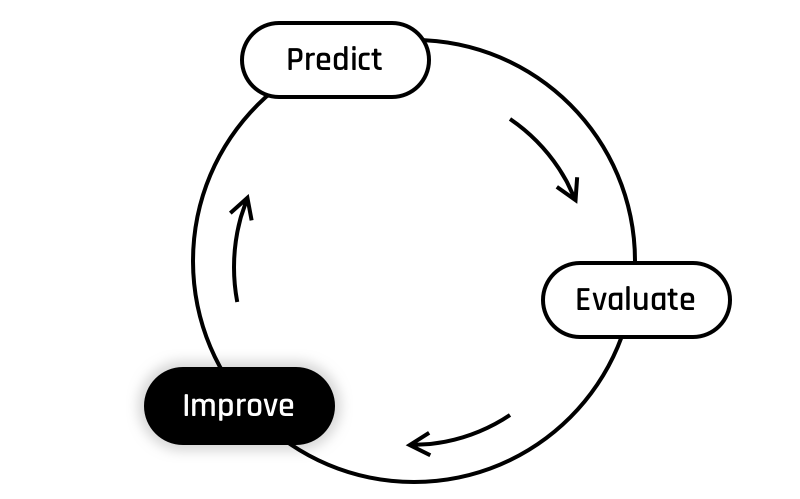
\includegraphics[scale=0.25]{assets/Improve.png}
    %\caption{The Learning Cycle: Improve}
\end{figure}
\noindent{To derive the gradient of the regularized loss function, $\nabla(J)$ 
you have to change a bit the formula of the unregularized gradient.}\\
\\
Given the fact that we are not penalizing $\theta_0$, the formula will remain 
the same as before for this parameter. For the other parameters ($\theta_1, \dots, \theta_n$),
 we must add the partial derivative of the regularization term: $\lambda \theta_j$.\\
\\
Therefore, we get:
$$
\nabla(J)_0 = \frac{1}{m}\sum_{i=1}^{m}(h_\theta(x^{(i)}) - y^{(i)})
$$
$$
\nabla(J)_j = \frac{1}{m}\left(\sum_{i=1}^{m}(h_\theta(x^{(i)}) - y^{(i)})x_j^{(i)} + \lambda \theta_j\right) \text{ for j = 1, ..., n}
$$
\\
Where:  
\begin{itemize}
    \item $\nabla(J)_j$ is the j$^\text{th}$ component of the gradient vector $\nabla(J)$
    \item $m$ is the number of training examples used
    \item $h_\theta(x^{(i)})$ is the model's prediction for the i$^\text{th}$ training example
    \item $x^{(i)}$ is the feature vector of the i$^\text{th}$ training example
    \item $y^{(i)}$ is the expected target value for the i$^\text{th}$ example
    \item $\lambda$ is a constant, the regularization hyperparameter
    \item $\theta_j$ is the j$^\text{th}$ parameter of the $\theta$ vector
\end{itemize}
\bigskip
Which can be vectorized as:
$$
\nabla(J) = \frac{1}{m} [X'^T(h_\theta(X) - y) + \lambda \theta']
$$  
\\
Where:  
\begin{itemize}
    \item $\nabla(J)$ is a vector of length $(n + 1)$, the gradient vector
    \item $m$ is the number of training examples used
    \item $X$ is a matrix of dimension $(m \times n)$, the design matrix
    \item $X'$ is a matrix of dimension $(m \times (n + 1))$, the design matrix onto 
    which a column of ones is added as a first column
    \item $y$ is a vector of length $m$, the vector of expected values
    \item $h_\theta(X)$ is a vector of length $m$, the vector of predicted values
    \item $\lambda$ is a constant
    \item $\theta$ is a vector of length $(n + 1)$, the parameter vector
    \item $\theta'$ is a vector of length $(n + 1)$, constructed using the following rules:
\end{itemize}

$$
\begin{matrix}
\theta'_0 & =  0 \\
\theta'_j & =  \theta_j & \text{ for } j = 1, \dots, n\\    
\end{matrix}
$$

% =============================================== %
\subsection*{Linear Gradient vs Logistic Gradient}
% ----------------------------------------------- %
As before, we draw your attention on the only difference between the linear regression's 
and the logistic regression's gradient equations: \textbf{the hypothesis function} $h_\theta(X)$.
\begin{itemize}
    \item In the linear regression: $h_\theta(X) = X'\theta$
    \item In the logistic regression: $h_\theta(X) = \text{sigmoid}(X'\theta)$
\end{itemize}

\newpage
\turnindir{ex04}
\exnumber{04}
\exfiles{log\_gradient.py}
\exforbidden{any function that performs derivatives for you}
\makeheaderfilesforbidden


% ================================= %
\section*{Objective}
% --------------------------------- %
Understand and manipulate the concept of gradient in case of logistic formulation.
You must implement the following formula as a function:  

$$
\begin{matrix}
\nabla(J)_0 &  = &\cfrac{1}{m}\sum_{i=1}^{m}(h_{\theta}(x^{(i)}) - y^{(i)}) & \\
\nabla(J)_j & = &\cfrac{1}{m}\sum_{i=1}^{m}(h_{\theta}(x^{(i)}) - y^{(i)})x_{j}^{(i)} & \text{ for j = 1, ..., n}    
\end{matrix}
$$

Where:
\begin{itemize}
  \item $\nabla(J)$ is a vector of size $(n + 1)$, the gradient vector.
  \item $\nabla(J)_j$ is the j$^\text{th}$ component of $\nabla(J)$, the partial derivative of $J$ with respect to $\theta_j$.
  \item $y$ is a vector of dimension $m$, the vector of expected values.
  \item $y^{(i)}$ is a scalar, the i$^\text{th}$ component of vector $y$.
  \item $x^{(i)}$ is the feature vector of the i$^\text{th}$ example.
  \item $x^{(i)}_j$ is a scalar, the j$^\text{th}$ feature value of the i$^\text{th}$ example.
  \item $h_{\theta}(x^{(i)})$ is a scalar, the model's estimation of $y^{(i)}$.
\end{itemize}

Remember that with logistic regression, the hypothesis is slightly different:  

$$
h_{\theta}(x^{(i)}) = sigmoid( \theta \cdot x'^{(i)})
$$

% ================================= %
\section*{Instructions}
% --------------------------------- %
In the \texttt{log\_gradient.py} file, write the following function as per the instructions below:

\begin{minted}[bgcolor=darcula-back,formatcom=\color{lightgrey},fontsize=\scriptsize]{python}
def log_gradient(x, y, theta):
    """Computes a gradient vector from three non-empty numpy.ndarray, with a for-loop. The three arrays must have compatible dimensions.
    Args:
      x: has to be an numpy.ndarray, a matrix of shape m * n.
      y: has to be an numpy.ndarray, a vector of shape m * 1.
      theta: has to be an numpy.ndarray, a vector of shape (n + 1) * 1.
    Returns:
      The gradient as a numpy.ndarray, a vector of shape n * 1, containing the result of the formula for all j.
      None if x, y, or theta are empty numpy.ndarray.
      None if x, y and theta do not have compatible dimensions.
    Raises:
      This function should not raise any Exception.
    """
    ... Your code ...
\end{minted}

% ================================= %
\section*{Examples}
% ================================= %
\begin{minted}[bgcolor=darcula-back,formatcom=\color{lightgrey},fontsize=\scriptsize]{python}
# Example 1:
y1 = np.array([1]).reshape((-1, 1))
x1 = np.array([4]).reshape((-1, 1))
theta1 = np.array([[2], [0.5]])

log_gradient(x1, y1, theta1)
# Output:
array([[-0.01798621],
       [-0.07194484]])

# Example 2: 
y2 = np.array([[1], [0], [1], [0], [1]])
x2 = np.array([[4], [7.16], [3.2], [9.37], [0.56]])
theta2 = np.array([[2], [0.5]])

log_gradient(x2, y2, theta2)
# Output:
array([[0.3715235 ],
       [3.25647547]])

# Example 3: 
y3 = np.array([[0], [1], [1]])
x3 = np.array([[0, 2, 3, 4], [2, 4, 5, 5], [1, 3, 2, 7]])
theta3 = np.array([[-2.4], [-1.5], [0.3], [-1.4], [0.7]])

log_gradient(x3, y3, theta3)
# Output:
array([[-0.55711039],
       [-0.90334809],
       [-2.01756886],
       [-2.10071291],
       [-3.27257351]])
\end{minted}
% ===========================(fin ex 04)         %
% ============================================== %
\newpage
% ============================================== %
% ===========================(start ex 05)       %
\chapter{Exercise 05}
\extitle{Vectorized Logistic Gradient}
%******************************************************************************%
%                                                                              %
%                                 Interlude                                    %
%                         for Machine Learning module                          %
%                                                                              %
%******************************************************************************%

\section*{Interlude - Normalization}

The values inside the $x$ vector can vary quite a lot in magnitude,
depending on the type of data you are working with.
For example, if your dataset contains distances between planets in km, the numbers will be huge.
On the other hand, if you are working with planet masses expressed as a fraction of the solar system's total mass, the numbers will be very small (between 0 and 1).
Both cases may slow down convergence in Gradient Descent (or even sometimes prevent convergence at all).
To avoid that kind of situation, normalization is a very effective way to proceed.


The idea behind this technique is straightforward: \textbf{scaling the data}.  


With normalization, you can transform your $x$ vector into a new $x'$ vector whose values range between $[-1, 1]$ more or less. Doing this allows you to see much more easily how a training example compares to the other ones:
\begin{itemize}
    \item If an $x'$ value is close to $1$, you know it's among the largest in the dataset
    \item If an $x'$ value is close to $0$, you know it's close to the median
    \item If an $x'$ value is close to $-1$, you know it's among the smallest
\end{itemize}

So with the upcoming normalization techniques, you'll be able to map your data to two different value ranges: $[0, 1]$ or $[-1, 1]$. Your algorithm will like it and thank you for it.  

\newpage
\turnindir{ex05}
\exnumber{05}
\exfiles{vec\_log\_gradient.py}
\exforbidden{any function that performs derivatives for you}
\makeheaderfilesforbidden

% ================================= %
\section*{Objective}
% --------------------------------- %
Understand and manipulate the gradient in the context of logistic formulation.\\
\\
You must implement the following formula as a function:

$$
\nabla(J) = \cfrac{1}{m} X'^T(h_\theta(X) - y)
$$  
\\
Where:  
\begin{itemize}
  \item $\nabla(J)$ is the gradient vector of length $(n + 1)$
  \item $X'$ is a matrix of dimensions $(m \times (n + 1))$, the design matrix onto which a column of ones was added as the first column
  \item $X'^T$ means the matrix has been transposed
  \item $h_\theta(X)$ is a vector of length $m$, the vector of predicted values
  \item $y$ is a vector of dimension $m$, the vector of expected values
\end{itemize}


% ================================= %
\section*{Instructions}
% --------------------------------- %
In the \texttt{vec\_log\_gradient.py} file, write the following function as per the instructions given below:
\\
\par
\begin{minted}[bgcolor=darcula-back,formatcom=\color{lightgrey},fontsize=\scriptsize]{python}
def vec_log_gradient(x, y, theta):
    """Computes a gradient vector from three non-empty numpy.ndarray, without any for-loop. The three arrays must have compatible shapes.
    Args:
      x: has to be an numpy.ndarray, a matrix of shape m * n.
      y: has to be an numpy.ndarray, a vector of shape m * 1.
      theta: has to be an numpy.ndarray, a vector (n +1) * 1.
    Returns:
      The gradient as a numpy.ndarray, a vector of shape n * 1, containg the result of the formula for all j.
      None if x, y, or theta are empty numpy.ndarray.
      None if x, y and theta do not have compatible shapes.
    Raises:
      This function should not raise any Exception.
    """
    ... Your code ...
\end{minted}


% ================================= %
\section*{Examples}
% --------------------------------- %
\begin{minted}[bgcolor=darcula-back,formatcom=\color{lightgrey},fontsize=\scriptsize]{python}
# Example 1:
y1 = np.array([1]).reshape((-1, 1))
x1 = np.array([4]).reshape((-1, 1))
theta1 = np.array([[2], [0.5]])

vec_log_gradient(x1, y1, theta1)
# Output:
array([[-0.01798621],
       [-0.07194484]])

# Example 2: 
y2 = np.array([[1], [0], [1], [0], [1]])
x2 = np.array([[4], [7.16], [3.2], [9.37], [0.56]])
theta2 = np.array([[2], [0.5]])

vec_log_gradient(x2, y2, theta2)
# Output:
array([[0.3715235 ],
       [3.25647547]])

# Example 3: 
y3 = np.array([[0], [1], [1]])
x3 = np.array([[0, 2, 3, 4], [2, 4, 5, 5], [1, 3, 2, 7]])
theta3 = np.array([[-2.4], [-1.5], [0.3], [-1.4], [0.7]])

vec_log_gradient(x3, y3, theta3)
# Output:
array([[-0.55711039],
       [-0.90334809],
       [-2.01756886],
       [-2.10071291],
       [-3.27257351]])
\end{minted}
% ===========================(fin ex 05)         %
% ============================================== %
\newpage
% ============================================== %
% ===========================(start ex 06)       %
\chapter{Exercise 06}
\extitle{Logistic Regression}
%%******************************************************************************%
%                                                                              %
%                                 Interlude                                    %
%                         for Machine Learning module                          %
%                                                                              %
%******************************************************************************%

\section*{Interlude - Evaluate}

\begin{figure}[h!]
  \centering
  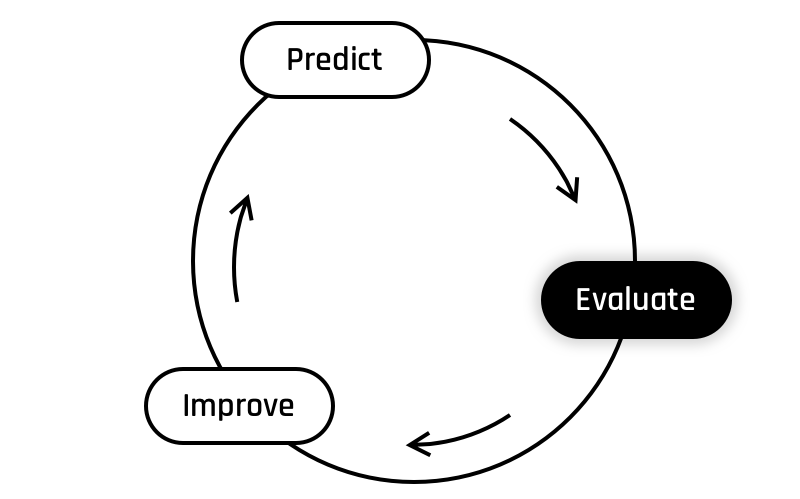
\includegraphics[scale=0.25]{assets/Evaluate.png}
  % \caption{cycle evaluate}
\end{figure}

\subsection*{Introducing the loss function}

How good is our model?  
It is hard to say just by simply looking at the plots!
We can clearly observe that certain regression lines seem to fit the data better than others, but it would be convenient to find a way to measure it. 

\begin{figure}[h!]
  \centering
  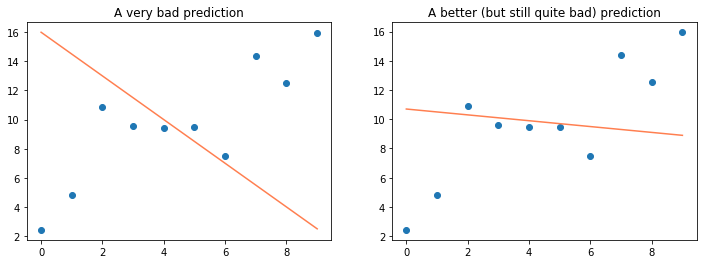
\includegraphics[scale=0.55]{assets/bad_prediction.png}
  \caption{bad prediction}
\end{figure}

To evaluate our model, we are going to use a \textbf{metric} called \textbf{the loss function} (sometimes called \textbf{cost function}).\\
\newline
The loss function tells us how bad our model is performing, how much it \textit{costs} us to use it, how much information we \textit{lose} when we use it.
If the model is good, we won't lose that much; if it's terrible instead, we will have a high loss!

The metric you choose will deeply impact the evaluation (and therefore also the training) of your model.

A frequent way to evaluate the performance of a regression model is to measure the distance between each predicted value ($\hat{y}^{(i)}$) and the real value it tries to predict (${y}^{(i)}$). The distances are then squared, and averaged to get one single metric, denoted $J$:

$$
J(\theta) = \frac{1}{2m}\sum_{i=1}^{m}(\hat{y}^{(i)} - y^{(i)})^2
$$

The smaller, the better! 

\begin{figure}[h!]
  \centering
  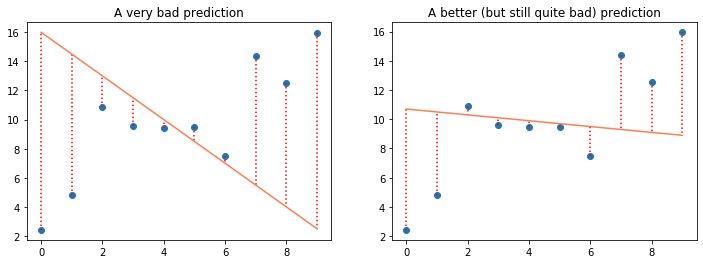
\includegraphics[scale=0.55]{assets/bad_pred_with_distance.png}
  \caption{bad prediction with distance}
\end{figure}

%\newpage
\turnindir{ex06}
\exnumber{06}
\exfiles{my\_logistic\_regression.py}
\exforbidden{sklearn}
\makeheaderfilesforbidden

% ================================= %
\section*{Objective}
% --------------------------------- %
The time to use everything you built so far has come! Demonstrate your knowledge by implementing a logistic regression classifier using the gradient descent algorithm.
You must have seen the power of \texttt{numpy} for vectorized operations. Well let's make something more concrete with that.

You may have to take a look at Scikit-Learn's implementation of logistic regression and noticed that the \textbf{sklearn.linear\_model.LogisticRegression} class offers a lot of options.

The goal of this exercise is to make a simplified but nonetheless useful and powerful version, with fewer options.

% ================================= %
\section*{Instructions}
% --------------------------------- %
In the \texttt{my\_logistic\_regression.py} file, write a \texttt{MyLogisticRegression} class as in the instructions below:

\begin{minted}[bgcolor=darcula-back,formatcom=\color{lightgrey},fontsize=\scriptsize]{python}
class MyLogisticRegression():
	"""
	Description:
		My personnal logistic regression to classify things.
	"""
    def __init__(self, theta, alpha=0.001, max_iter=1000):
        self.alpha = alpha
        self.max_iter = max_iter
        self.theta = theta
        ... Your code here ...

	... other methods ...
\end{minted}

You will add at least the following methods:
\begin{itemize}
  \item \texttt{predict\_(self, x)}
  \item \texttt{loss\_elem\_(self, y, yhat)}
  \item \texttt{loss\_(self, y, yhat)}
  \item \texttt{fit\_(self, x, y)}
\end{itemize}

You have already written these functions, you will just need few adjustments so that they all work well within your \texttt{MyLogisticRegression} class.

% ================================= %
\subsection*{Examples}
% --------------------------------- %

\begin{minted}[bgcolor=darcula-back,formatcom=\color{lightgrey},fontsize=\scriptsize]{python}
import numpy as np
from my_logistic_regression import MyLogisticRegression as MyLR
X = np.array([[1., 1., 2., 3.], [5., 8., 13., 21.], [3., 5., 9., 14.]])
Y = np.array([[1], [0], [1]])
thetas = np.array([[2], [0.5], [7.1], [-4.3], [2.09]])
mylr = MyLR(thetas)

# Example 0:
mylr.predict_(X)
# Output:
array([[0.99930437],
       [1.        ],
       [1.        ]])

# Example 1:
mylr.loss_(X,Y)
# Output:
11.513157421577002

# Example 2:
mylr.fit_(X, Y)
mylr.theta
# Output:
array([[ 2.11826435]
       [ 0.10154334]
       [ 6.43942899]
       [-5.10817488]
       [ 0.6212541 ]])

# Example 3:
mylr.predict_(X)
# Output:
array([[0.57606717]
       [0.68599807]
       [0.06562156]])

# Example 4:
mylr.loss_(X,Y)
# Output:
1.4779126923052268
\end{minted}
% ===========================(fin ex 06)         %
% ============================================== %
\newpage
% ============================================== %
% ===========================(start ex 07)       %
\chapter{Exercise 07}
\extitle{Practicing Logistic Regression}
%%******************************************************************************%
%                                                                              %
%                                 Interlude                                    %
%                         for Machine Learning module                          %
%                                                                              %
%******************************************************************************%

% =============================================== %
\section*{Interlude - Introducing Polynomial Models}
% ----------------------------------------------- %

You probably noticed that the method we use is called \textit{linear regression} for a reason:
the model generates all of its predictions on a straight line.
However, we often encounter features that do not have a linear relationship with the predicted variable,
like in the figure below:

\begin{figure}[!h]
    \centering
    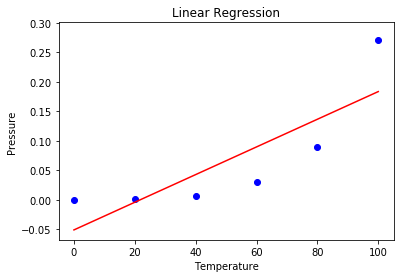
\includegraphics[scale=0.6]{assets/polynomial_straight_line.png}
    \caption{Non-linear relationship}
\end{figure}

In that case, we are stuck with a straight line that cannot fit the data points properly.
In this example, what if we could express $y$ not as a function of $x$, but also of $x^2$, and maybe even $x^3$ and $x^4$?
We could make a hypothesis that draws a nice \textbf{curve} that would better fit the data.
That's where polynomial features can help!

% =============================================== %
\section*{Interlude - Polynomial features}
% ----------------------------------------------- %
First we get to do some \textit{feature engineering}.
We create new features by raising our initial $x$ feature to the power of 2, and then 3, 4... as far as we want to go.
For each new feature we need to create a new column in the dataset.

% =============================================== %
\section*{Interlude - Polynomial Hypothesis}
% ----------------------------------------------- %
Now that we created our new features, we can combine them in a linear hypothesis that looks just the same as what we're used to:

$$
\hat{y} = \theta_0 + \theta_1 x  +\theta_2 x^{2} + \dots + \theta_n x^{n}
$$  

It's a little strange because we are building a linear combination, not with different features but with different powers of the same feature.
This is a first way of introducing non-linearity in a regression model!
%\newpage
\turnindir{ex07}
\exnumber{07}
\exfiles{mono\_log.py, multi\_log.py}
\exforbidden{sklearn}
\makeheaderfilesforbidden


% ================================= %
\section*{Objective}
% --------------------------------- %
Now it's time to test your Logistic Regression Classifier on real data!  
You will use the \textbf{solar\_system\_census\_dataset}. 

% ================================= %
\section*{Instructions}
% --------------------------------- %
Some words about the dataset:
\begin{itemize}
  \item You will work with data from the last Solar System Census.
  \item The dataset is divided in two files which can be found in the \texttt{resources} folder: \texttt{solar\_system\_census.csv} and \texttt{solar\_system\_census\_planets.csv}.
  \item The first file contains biometric information such as the height, weight, and bone density of several Solar System citizens.
  \item The second file contains the homeland of each citizen, indicated by its Space Zipcode representation (i.e. one number for each planet... :)).
\end{itemize}

\newpage

As you should know, Solar citizens come from four registered areas (zipcodes): 
\begin{itemize}
  \item The flying cities of Venus (0), 
  \item United Nations of Earth (1), 
  \item Mars Republic (2), 
  \item The Asteroids' Belt colonies (3).
\end{itemize}


You are expected to produce 2 programs that will use Logistic Regression to predict from which planet each citizen comes from, based on the other variables found in the census dataset.  

But wait... what? There are four different planets! How do you make a classifier discriminate between 4 categories? Let's go step by step...


% ================================= %
\section*{One Label to Discriminate Them All}
% --------------------------------- %
You already wrote a Logistic Regression Classifier that can discriminate between two classes.
We can use it to solve the problem!
Let's start by having it discriminate between citizens who come from your favorite planet and everybody else!

Your program (in \texttt{mono\_log.py}) will:
\begin{enumerate}
  \item Take an argument: \texttt{--zipcode=x} with $x$ being $0$, $1$, $2$ or $3$.
        If no argument, usage will be displayed.
  \item Split the dataset into a training and a test set.
  \item Select your favorite Space Zipcode and generate a new \texttt{numpy.array} to label each citizen according to your new selection criterion:
  \begin{itemize}
    \item $1$ if the citizen's zipcode corresponds to your favorite planet.
    \item $0$ if the citizen has another zipcode.
  \end{itemize}
  \item Train a logistic model to predict if a citizen comes from your favorite planet or not, using your brand new label.
  \item Calculate and display the fraction of correct predictions over the total number of predictions based on the test set.
  \item Plot 3 scatter plots (one for each pair of citizen features) with the dataset and the final prediction of the model.
\end{enumerate}

\begin{quote}
  You can use normalization on your dataset. The question is: Should you?
\end{quote}

You now have a model that can discriminate between citizens that come from one specific planet and everyone else.
It's a first step, a good one, but we still have work to do before we can classify citizens among four planets!

So how does \textbf{Multiclass Logistic Regression} work?  

% ================================= %
\section*{One Versus All}
% --------------------------------- %
The idea now is to apply what is called \textbf{one-versus-all classification}.
It's quite straightforward:

Your program (in \texttt{multi\_log.py}) will:
\begin{enumerate}
  \item Split the dataset into a training and a test set.
  \item Train 4 logistic regression classifiers to discriminate each class from the others (the way you did in part one).
  \item Predict for each example the class according to each classifiers and select the one with the highest output probability.
  \item Calculate and display the fraction of correct predictions over the total number of predictions based on the test set.
  \item Plot 3 scatter plots (one for each pair of citizen features) with the dataset and the final prediction of the model.
\end{enumerate}


% ================================= %
\section*{Examples}
% --------------------------------- %
If a cititzen got the following classification probabilities: 
\begin{itemize}
  \item Planet 0 vs all: $0.38$
  \item Planet 1 vs all: $0.51$
  \item Planet 2 vs all: $0.12$
  \item Planet 3 vs all: $0.89$
\end{itemize}

Then the citizen should be classified as coming from \textit{Planet 3}. 
% ===========================(fin ex 07)         %
% ============================================== %
\newpage
% ============================================== %
% ===========================(start ex 08)       %
\chapter{Exercise 08}
\extitle{Other metrics}
%******************************************************************************%
%                                                                              %
%                                 Interlude                                    %
%                         for Machine Learning module                          %
%                                                                              %
%******************************************************************************%

\section*{Interlude - Fifty Shades of Linear Algebra}

In the last exercise, we implemented the loss function in two subfunctions.
It worked, but it's not very pretty.
What if we could do it all in one step, with linear algebra?   

As we did with the hypothesis, we can use a vectorized equation to improve the calculations of the loss function.

So now let's look at how squaring and averaging can be performed (more or less) in a single matrix multiplication!

$$
J(\theta) = \frac{1}{2m}\sum_{i=1}^{m}(\hat{y}^{(i)} - y^{(i)})^2
$$
$$
J(\theta) = \frac{1}{2m}\sum_{i=1}^{m}[(\hat{y}^{(i)} - y^{(i)}) (\hat{y}^{(i)} - y^{(i)})]
$$

Now, if we apply the definition of the dot product:

$$
J(\theta) = \frac{1}{2m}(\hat{y} - y) \cdot(\hat{y}- y)
$$
\newpage
\turnindir{ex08}
\exnumber{08}
\exfiles{other\_metrics.py}
\exforbidden{None}
\makeheaderfilesforbidden

% ================================= %
\section*{Objective}
% --------------------------------- %
Understand and experiment with the classification criteria (TP, FP, ...) and metrics.\\
\\
The goal of this exercise is to write four metric functions (which are also 
available in \textbf{sklearn.metrics}) and to understand what they measure and how they are designed.\\
\\
You must implement the following fomulas: 

$$
\text{accuracy} = \frac{\text{tp} + \text{tn}}{\text{tp} + \text{fp} + \text{tn} + \text{fn}}
$$
$$
\text{precision} = \frac{\text{\text{tp}}}{\text{tp} + \text{fp}}
$$
$$
\text{recall} = \frac{\text{tp}}{\text{tp} + \text{fn}}
$$
$$
\text{F1score} = \frac{2 \times \text{precision} \times \text{recall}}{\text{precision} + \text{recall}}
$$
Where:
\begin{itemize}
  \item $\text{tp}$ is the number of \textbf{true positives}
  \item $\text{fp}$ is the number of \textbf{false positives}
  \item $\text{tn}$ is the number of \textbf{true negatives}
  \item $\text{fn}$ is the number of \textbf{false negatives}
\end{itemize}
\newpage
% ================================= %
\section*{Instructions}
% --------------------------------- %
For the sake of simplicity, we will only ask you to use two parameters.\\
\\
In the \texttt{other\_metrics.py} file, write the following functions as per 
the instructions given below:\\
\\
\begin{minted}[bgcolor=darcula-back,formatcom=\color{lightgrey},fontsize=\scriptsize]{python}
def accuracy_score_(y, y_hat):
    """
    Compute the accuracy score.
    Args:
        y:a numpy.ndarray for the correct labels
        y_hat:a numpy.ndarray for the predicted labels
    Returns: 
        The accuracy score as a float.
        None on any error.
    Raises:
        This function should not raise any Exception.
    """
    ... Your code ...

def precision_score_(y, y_hat, pos_label=1):
    """
    Compute the precision score.
    Args:
        y:a numpy.ndarray for the correct labels
        y_hat:a numpy.ndarray for the predicted labels
        pos_label: str or int, the class on which to report the precision_score (default=1)
    Returns: 
        The precision score as a float.
        None on any error.
    Raises:
        This function should not raise any Exception.
    """
    ... Your code ...

def recall_score_(y, y_hat, pos_label=1):
    """
    Compute the recall score.
    Args:
        y:a numpy.ndarray for the correct labels
        y_hat:a numpy.ndarray for the predicted labels
        pos_label: str or int, the class on which to report the precision_score (default=1)
    Returns: 
        The recall score as a float.
        None on any error.
    Raises:
        This function should not raise any Exception.
    """
    ... Your code ...

def f1_score_(y, y_hat, pos_label=1):
    """
    Compute the f1 score.
    Args:
        y:a numpy.ndarray for the correct labels
        y_hat:a numpy.ndarray for the predicted labels
        pos_label: str or int, the class on which to report the precision_score (default=1)
    Returns: 
        The f1 score as a float.
        None on any error.
    Raises:
        This function should not raise any Exception.
    """
    ... Your code ...
\end{minted}

% ================================= %
\section*{Examples}
% --------------------------------- %
\begin{minted}[bgcolor=darcula-back,formatcom=\color{lightgrey},fontsize=\scriptsize]{python}
import numpy as np
from sklearn.metrics import accuracy_score, precision_score, recall_score, f1_score   

# Example 1:
y_hat = np.array([1, 1, 0, 1, 0, 0, 1, 1]).reshape((-1, 1))
y = np.array([1, 0, 0, 1, 0, 1, 0, 0]).reshape((-1, 1))

# Accuracy
## your implementation
accuracy_score_(y, y_hat)
## Output:
0.5
## sklearn implementation
accuracy_score(y, y_hat)
## Output:
0.5

# Precision
## your implementation
precision_score_(y, y_hat)
## Output:
0.4
## sklearn implementation
precision_score(y, y_hat)
## Output:
0.4

# Recall
## your implementation
recall_score_(y, y_hat)
## Output:
0.6666666666666666
## sklearn implementation
recall_score(y, y_hat)
## Output:
0.6666666666666666

# F1-score
## your implementation
f1_score_(y, y_hat)
## Output:
0.5
## sklearn implementation
f1_score(y, y_hat)
## Output:
0.5
\end{minted}

\begin{minted}[bgcolor=darcula-back,formatcom=\color{lightgrey},fontsize=\scriptsize]{python}
# Example 2:
y_hat = np.array(['norminet', 'dog', 'norminet', 'norminet', 'dog', 'dog', 'dog', 'dog'])
y = np.array(['dog', 'dog', 'norminet', 'norminet', 'dog', 'norminet', 'dog', 'norminet'])

# Accuracy
## your implementation
accuracy_score_(y, y_hat)
## Output:
0.625
## sklearn implementation
accuracy_score(y, y_hat)
## Output:
0.625

# Precision
## your implementation
precision_score_(y, y_hat, pos_label='dog')
## Output:
0.6
## sklearn implementation
precision_score(y, y_hat, pos_label='dog')
## Output:
0.6

# Recall
## your implementation
recall_score_(y, y_hat, pos_label='dog')
## Output:
0.75
## sklearn implementation
recall_score(y, y_hat, pos_label='dog')
## Output:
0.75

# F1-score
## your implementation
f1_score_(y, y_hat, pos_label='dog')
## Output:
0.6666666666666665
## sklearn implementation
f1_score(y, y_hat, pos_label='dog')
## Output:
0.6666666666666665
\end{minted}

\begin{minted}[bgcolor=darcula-back,formatcom=\color{lightgrey},fontsize=\scriptsize]{python}
# Example 3:
y_hat = np.array(['norminet', 'dog', 'norminet', 'norminet', 'dog', 'dog', 'dog', 'dog'])
y = np.array(['dog', 'dog', 'norminet', 'norminet', 'dog', 'norminet', 'dog', 'norminet'])

# Precision
## your implementation
precision_score_(y, y_hat, pos_label='norminet')
## Output:
0.6666666666666666
## sklearn implementation
precision_score(y, y_hat, pos_label='norminet')
## Output:
0.6666666666666666

# Recall
## your implementation
recall_score_(y, y_hat, pos_label='norminet')
## Output:
0.5
## sklearn implementation
recall_score(y, y_hat, pos_label='norminet')
## Output:
0.5

# F1-score
## your implementation
f1_score_(y, y_hat, pos_label='norminet')
## Output:
0.5714285714285715
## sklearn implementation
f1_score(y, y_hat, pos_label='norminet')
## Output:
0.5714285714285715
\end{minted}

% ===========================(fin ex 08)         %
% ============================================== %
\newpage
% ============================================== %
% ===========================(start ex 09)       %
\chapter{Exercise 09}
\extitle{Confusion Matrix}
%%******************************************************************************%
%                                                                              %
%                                 Interlude                                    %
%                         for Machine Learning module                          %
%                                                                              %
%******************************************************************************%

% ============================================== %
\section*{Interlude - Lost in Overfitting}
% ---------------------------------------------- %

The two previous exercises lead you, dear reader, to a very dangerous territory: the realm of \textbf{overfitting}.\\
You did not see it coming but now, you are in a bad situation...\\
\\
By increasing the polynomial degree of your model, you increased its \textbf{complexity}.  
Is it wrong?
Not always.
Some models are indeed very complex because the relationships they represent are very complex as well.\\
\\
But, if you look at the plots for the previous exercise's \textit{best model}, you should feel that something is wrong...\\
\\
% ============================================== %
\section*{Interlude - Something is rotten in the state of our model...}
% ---------------------------------------------- %
Take a look at the following plot. 

\begin{figure}[!h]
    \centering
    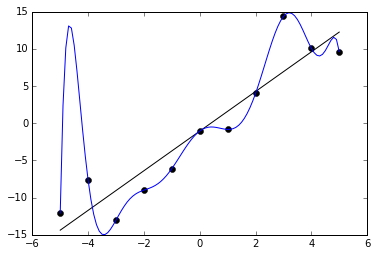
\includegraphics[scale=0.6]{assets/overfitt.png}
    \caption{Overfitting hypothesis}
\end{figure}

You can see that the prediction line fits each data point perfectly, but completely misses out on capturing the relationship between $x$ and $y$ properly.
And now, if we add some brand new data points to the dataset, we see that the predictions on those new examples are way off.

\begin{figure}[!h]
    \centering
    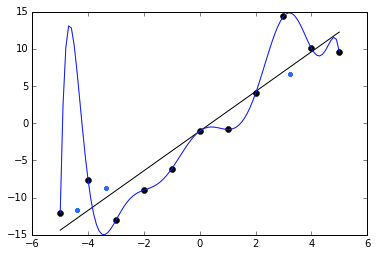
\includegraphics[scale=0.6]{assets/overfitt_with_dots.png}
    \caption{Generalization errors resulting from overfitting}
\end{figure}
This situation is called overfitting, because the model is doing an excessively good job at fitting the data.
It is literally bending over backward to account for the data's mini details.
But most of the data's irregularities are just noise, and they should in fact be ignored.
So because the model overfits, it can't generalize to new data.

% ============================================== %
\section*{Interlude - The training set, the test set, and the happy data scientist}
% ---------------------------------------------- %
To be able to detect overfitting, \textbf{you should always evaluate your model on new data}.\\
\\
New data means, data that your model hasn't seen during training.\\
\\
It's the only way to make sure your model isn't \textit{recalling}.
To do so, now and forever, you must always divide your dataset in (at least) two parts: one for the training, and one for the evaluation of your model.
%\newpage
\turnindir{ex09}
\exnumber{09}
\exfiles{confusion\_matrix.py}
\exforbidden{None}
\makeheaderfilesforbidden

% ================================= %
\section*{Objective}
% --------------------------------- %
Manipulation of confusion matrix concept.\
The goal of this exercise is to reimplement the function \texttt{confusion\_matrix} available in \textbf{sklearn.metrics} and to learn what does the confusion matrix represent.

% ================================= %
\section*{Instructions}
% --------------------------------- %
For the sake of simplicity, we will only ask you to use three parameters.
Be careful to respect the order, true labels are rows and predicted labels are columns:

\begin{center}
  \begin{tabular}{|c|c|c|c|}
    \cline{3-4}
    \multicolumn{2}{c|}{\multirow{2}{*}{}}  & \multicolumn{2}{|c|}{predicted labels} \\ \cline{3-4}
    \multicolumn{2}{c|}{}       & label 1 & label 2 \\
    \hline
    \multirow{2}{*}{true label} & label 1 &         &         \\
    \cline{2-4}
                                & label 2 &         &         \\
    \hline
  \end{tabular}
\end{center}

In the \texttt{confusion\_matrix.py} file, write the following function as per the instructions below:

\begin{minted}[bgcolor=darcula-back,formatcom=\color{lightgrey},fontsize=\scriptsize]{python}
def confusion_matrix_(y_true, y_hat, labels=None):
    """
    Compute confusion matrix to evaluate the accuracy of a classification.
    Args:
        y_true: numpy.ndarray for the correct labels
        y_hat: numpy.ndarray for the predicted labels
        labels: Optional, a list of labels to index the matrix.
                This may be used to reorder or select a subset of labels. (default=None)
    Returns: 
        The confusion matrix as a numpy ndarray.
        None on any error.
    Raises:
        This function should not raise any Exception.
    """
    ... Your code ...
\end{minted}


% ================================= %
\section*{Examples}
% --------------------------------- %
\begin{minted}[bgcolor=darcula-back,formatcom=\color{lightgrey},fontsize=\scriptsize]{python}
import numpy as np
from sklearn.metrics import confusion_matrix

y_hat = np.array([['norminet'], ['dog'], ['norminet'], ['norminet'], ['dog'], ['bird']])
y = np.array([['dog'], ['dog'], ['norminet'], ['norminet'], ['dog'], ['norminet']])

# Example 1: 
## your implementation
confusion_matrix_(y, y_hat)
## Output:
array([[0 0 0]
       [0 2 1]
       [1 0 2]])
## sklearn implementation
confusion_matrix(y, y_hat)
## Output:
array([[0 0 0]
       [0 2 1]
       [1 0 2]])

# Example 2:
## your implementation
confusion_matrix_(y, y_hat, labels=['dog', 'norminet'])
## Output:
array([[2 1]
       [0 2]])
## sklearn implementation
confusion_matrix(y, y_hat, labels=['dog', 'norminet'])
## Output:
array([[2 1]
       [0 2]])
\end{minted}

\section{Optional part}

\subsection{Objective(s):}

For a more visual version, you can add an option to your previous confusion\_matrix\_ function to return a \texttt{pandas.DataFrame} instead of a numpy array.

\subsection{Instructions:}

In the \texttt{confusion\_matrix.py} file, write the following function as per the instructions below:

\begin{minted}[bgcolor=darcula-back,formatcom=\color{lightgrey},fontsize=\scriptsize]{python}
def confusion_matrix_(y_true, y_hat, labels=None, df_option=False):
    """
    Compute confusion matrix to evaluate the accuracy of a classification.
    Args:
        y_true: a numpy.ndarray for the correct labels
        y_hat: a numpy.ndarray for the predicted labels
        labels: optional, a list of labels to index the matrix. This may be used to reorder or select a subset of labels. (default=None)
        df_option: optional, if set to True the function will return a pandas DataFrame instead of a numpy array. (default=False)
    Returns: 
        Confusion matrix as a numpy ndarray or a pandas DataFrame according to df_option value.
        None on any error.
    Raises:
        This function should not raise any Exception.
    """
    ... Your code ...
\end{minted}

\section{Examples:}

\begin{minted}[bgcolor=darcula-back,formatcom=\color{lightgrey},fontsize=\scriptsize]{python}
import numpy as np
y_hat = np.array(['norminet', 'dog', 'norminet', 'norminet', 'dog', 'bird'])
y = np.array(['dog', 'dog', 'norminet', 'norminet', 'dog', 'norminet'])

# Example 1: 
confusion_matrix_(y, y_hat, df_option=True)
# Output:
           bird  dog  norminet
 bird         0    0         0
 dog          0    2         1
 norminet     1    0         2

# Example 2:
confusion_matrix_(y, y_hat, labels=['bird', 'dog'], df_option=True)
# Output:
           bird  dog
 bird         0    0
 dog          0    2
\end{minted}

\info{
  If you fail this exercise on your first attempt, Norminet will curse you forever.
  Yeah, you'd better do it right or you are in trouble my friend, big trouble!
}
% ===========================(fin ex 09)         %
% ============================================== %
\newpage
% ============================================== %
% ===========================(Conclusion)        %
\chapter{Conclusion - What you have learnt}

You are now done with the ML Bootcamp module03, well done !\\
\newline
Based on all the notions and problems
tackled today, you should be able to discuss and answer the following questions:

\begin{enumerate}
  \item Why do we use the logistic hypothesis for a classfication problem 
  rather than a linear hypothesis?
  \item What is the decision boundary?
  \item In the case we decide to use a linear hypothesis to tackle a 
  classification problem, why the classification of some data points can be
   altered by considering more examples (for example, extra data points with extrem ordinate)?
  \item In a one versus all classification approach, how many logisitic regressors do we
   need to distinguish between N classes?
  \item Can you explain the difference between accuracy and precision?
   What is the type I and type II errors?
  \item What is the interest of the F1-score?
\end{enumerate}

% ===========================(Conclusion)        %
% ============================================== %
\newpage
\section*{Contact}
% --------------------------------- %
You can contact 42AI by email: \href{mailto:contact@42ai.fr}{contact@42ai.fr}\\
\newline
Thank you for attending 42AI's Machine Learning Bootcamp module01 !

% ================================= %
\section*{Acknowledgements}
% --------------------------------- %
The Python \& ML bootcamps are the result of a collective effort. We would like to thank:\\
\begin{itemize}
  \item Maxime Choulika (cmaxime),
  \item Pierre Peigné (ppeigne),
  \item Matthieu David (mdavid),
  \item Quentin Feuillade--Montixi (qfeuilla, quentin@42ai.fr)
  \item Mathieu Perez (maperez, mathieu.perez@42ai.fr)
\end{itemize}
who supervised the creation and enhancements of the present transcription.\\
\begin{itemize}
  \item Louis Develle (ldevelle, louis@42ai.fr)
  \item Owen Roberts (oroberts)
  \item Augustin Lopez (aulopez)
  \item Luc Lenotre (llenotre)
  \item Amric Trudel (amric@42ai.fr)
  \item Benjamin Carlier (bcarlier@student.42.fr)
  \item Pablo Clement (pclement@student.42.fr)
  \item Amir Mahla (amahla, amahla@42ai.fr)
\end{itemize}
for your investment in the creation and development of these modules.\\
\begin{itemize}
    \item All prior participants who took a moment to provide their feedbacks, and help us improve these bootcamps !
  \end{itemize}

\vfill
\doclicenseThis

% ================================= %

\end{document}
